\section{Parallel Architecture Design}
In this section, we will have an analysis of the problem, starting from the sequential implementation, from which we will make some considerations about how to parallelize the process, in order to achieve better performance.

\subsection{Sequential implementation}
The sequential code consists in a loop in which the four operations are performed one after the other. In this case, all the computation is done by a single thread at a time.

Before the loop, two \texttt{cv::Mat} objects are created, called \texttt{grey\_frame} and \texttt{smoothed\_frame}; these variables will hold the results produced by the \texttt{to\_greyscale()} and the \texttt{smoothing()} functions respectively, and will be reused for each frame.
In the \texttt{smoothing()} function, we can also choose the filter that we want to use, among the four matrices proposed in the project description.\\
Instead, a \texttt{cv::Mat frame} will be used to store each frame loaded from the source video.

In the end, the \texttt{motion\_detection()} function, given the \texttt{processed\_background}, the current \texttt{smoothed\_frame} and a \texttt{threshold}, will increase the value of an integer variable \texttt{motion\_frames}, if there are enough different pixels between the two frames.

The loop will break when the loaded frame is empty, meaning that the source video is finished.

In Figure \ref{fig:seq_code} we have a representation of the workflow in the sequential implementation.

\begin{figure}[h]
    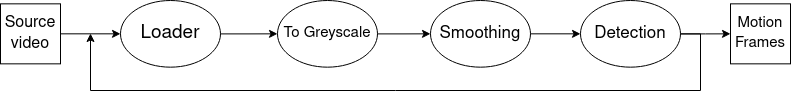
\includegraphics[width=\textwidth]{img/seq_code.png}
    \centering
    \caption{Scheme of the sequential implementation}
    \label{fig:seq_code}
\end{figure}

\pagebreak

\subsection{Analysis of the performance}
In order to study the problem from a theoretical point of view, we need to analyse the performance of the sequential code, taking into consideration the weight of each operation onto the overall computation time. To do so, a \emph{verbose} version of the sequential code was implemented, in which a different timer is used for each operation.\\
Since the \emph{Load} operation is provided by the \textbf{\emph{OpenCV}} library, it cannot be parallelized; therefore, it was not included in this analysis, also because it turns out that it takes a negligible time with respect to the other operations. 

\begin{wrapfigure}{r}{0.5\textwidth}
    \vspace{-6mm}
    \centering
    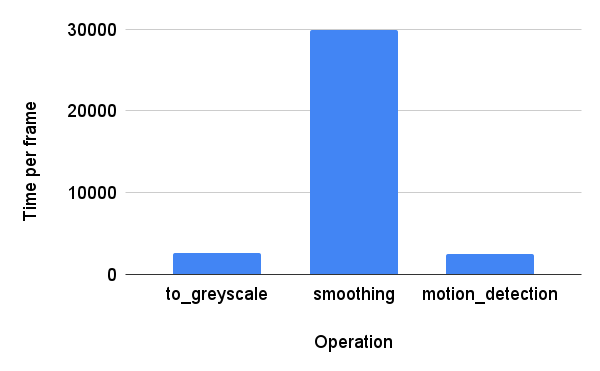
\includegraphics[width=0.5\textwidth]{img/seq_times_chart.png}
    \caption{Execution time of the sequential code}
    \label{fig:seq_times_chart}
\end{wrapfigure}

In Figure \ref{fig:seq_times_chart} there is a representation of the time needed by the sequential implementation to process one frame, divided for each operation. The times are expressed in  microseconds, and they are the result of an average of ten executions.\\
As we can see, the \texttt{smoothing()} operation is by far the most expensive one, since its execution time is one order of magnitude greater than the ones of the other two functions; in fact, it represents about the 85\% of the entire execution time. That is because this operation involves several convolutions, which is a costly operation, especially if computed on large matrices. For this reason, the \texttt{smoothing()} operation is the bottleneck of the process, and it is the one that needs to be parallelized to get a speedup.\\
On the other hand, the \texttt{to\_greyscale()} and \texttt{motion\_detection()} operations are much cheaper, since they basically require only a scan of the matrix plus simple operations on the pixels, which are, respectively, an addition and a division to compute the average and a subtraction to get the different pixels. 

\subsection{About the parallel implementation}
The first idea about how to implement a parallel version of this application was to have all the \emph{nw} workers processing a single frame per time step; that means to partition the frame into \emph{nw} subframes, have each worker processing its own section, and in the end perform the reconstruction of the entire frame. This version was abandoned because it was found to be slower than expected. That may be caused by the fact that a single operation on a subframe takes an amount of time which is too small, and that makes the overhead produced by the coordination of the threads to generate a noticeable slowdown.

Instead, the final version of the parallel implementation consists in a \emph{Farm} that process \emph{nw} frames in parallel. In the following section, we will see more in details the architecture of this implementation.